
%%%%%%%%%%%%%%%%%%%%%%%%%%%%%%%%%%%%%%%%%%%%%%%%%%%%%%%%%%%%%
%%%%%%%%%%%%%%%%%%%%%%%%%%%%%%%%%%%%%%%%%%%%%%%%%%%%%%%%%%%%%
%
%  %%%%%%%  %    %  %%%%%%  %%%%%%  %%%%%%%  %%%%%%%  %%%%%
%  %        %    %  %    %  %     %    %     %        %    %
%  %        %    %  %%%%%%  %     %    %     %        %    %
%  %        %%%%%%  %    %  %%%%%%     %     %%%%%    %%%%%
%  %        %    %  %    %  %          %     %        %    %
%  %%%%%%%  %    %  %    %  %          %     %%%%%%%  %     %
%
%%%%%%%%%%%%%%%%%%%%%%%%%%%%%%%%%%%%%%%%%%%%%%%%%%%%%%%%%%%%%
%%%%%%%%%%%%%%%%%%%%%%%%%%%%%%%%%%%%%%%%%%%%%%%%%%%%%%%%%%%%%
\chapter{Preliminary Examples}
\label{sec:examples}

% \begin{quote}
% {\em``I am pretty convinced that there is an ongoing reversal in the collective consciousness of mathematicians: the right hemispherical and homotopical picture of the world becomes the basic intuition, and if you want to get a discrete set, then you pass to the set of connected components of a space only defined up to homotopy.''}
% \begin{flushright} --- Yuri Manin~\cite{gelfand2009we} \end{flushright}
% \end{quote}
\begin{quote}
{\em``The content of a mathematical theory is never larger than the set of examples that are thoroughly understood.''}
\begin{flushright} --- Vladmir Arnol'd~\cite{arnol2004lectures} \end{flushright}
\end{quote}


Theories should be motivated by examples. In this chapter we develop the common themes these examples share. Broadly speaking, all sheaves are realized via local sections associated to a particular map. This principle is rigorously embodied by the \emph{\'etal\'e perspective}. Similarly, all cosheaves of sets are realized by connected components of the fiber of a map, embodied by the \emph{display perspective}, which is a generalization of the Reeb graph construction outlined in Definition~\ref{defn:reeb_graph}.

\section{Sheaves Model Sections}

Recall that if $f:Y\to X$ is a continuous map then a \textbf{section} is a continuous map $g:X\to Y$ such that $f(g(x))=x$ for all $x$. This definition has the property that $f$ is surjective. Sometimes a map admits a locally-defined section over a subset $U\subset X$, but not a global one. There is a sheaf that tracks this data.

\begin{defn}[Sheaf of Sections of a Map]\index{sheaf!of sections}
	Suppose $\pi:E\to X$ is a continuous map. Then we can associate a \textbf{sheaf of sections} to this map as follows:
	\[
	U\rightsquigarrow F(U):=\{s:U\to \pi^{-1}(U)\,\mathrm{continuous}\, | \pi(s(x))=x \}.
	\]
\end{defn}

Clearly, if $F(X)\neq \emptyset$, then we can answer positively the question ``Does $\pi:E\to X$ have a section?''
\[
\xymatrix{E\ar[d]_{\pi} \\ X \ar@/_/@{.>}[u]_{?}}
\]

To see why this is a pre-sheaf valued in $\dat=\Set$ note that what is assigned to an open set $U$ is a set of maps. A map whose domain of definition is $U$ can always be restricted to a smaller open subset $V\subset U$ to define a map on $V$. This process of restricting the domain of definition we write as $\rho_{V,U}(s):=s|_V$, which is what makes this assignment a pre-sheaf. 

Let us prove this defines a sheaf. Suppose $U\subset X$ and $\covU=\{U_i\}_{i\in\Lambda}$ is an arbitrary open cover of $U$. We must prove that the map
\[
F(U)\to F[\covU]:=\varprojlim(N(\covU)^{op}\to\Open(X)^{op}\to \Set)
\]
is an isomorphism.
Recall that the limit can be described in terms of products and equalizers. As such, every element of the limit is described by a collection of continuous sections $s_i:U_i\to \pi^{-1}(U_i)$, one for each element of the cover, such that on intersections $\rho_{ij,i}(s_i)=\rho_{ij,j}(s_j)$.\footnote{Here we have adopted the shorthand of referring to open sets via elements of the nerve.} The natural map from $F(U)$ to $F[\covU]$ simply takes a section $s\in F(U)$ to the collection of restricted sections $\{s_i:=s|_{U_i}\}$. If two sections over $U$ differ at a point $x$, then they will define different sections over $U_i\ni x$, thus the natural map is injective. To check surjectivity, note that an element in the limit defines a section over $U$ by setting $s(x)=s_i(x)$ if $x\in U_i$ and this will be continuous by the pasting lemma described at the beginning of Chapter~\ref{sec:abstract_sheaves}.

\begin{ex}
For a simple example, consider the projection onto the first coordinate $\pi_t:[0,1]\times [0,1]\to [0,1]$, which we regard as taking a time-space coordinate $(t,x)$ to its time coordinate $t$. There are lots of sections of this map. The map that assigns to each time $t$ a fixed position $p\in[0,1]$ defines a section, so there are uncountably many sections.

Now consider a different map that comes from restricting the time projection map to a subset $E\subseteq [0,1]\times[0,1]$, i.e. $\pi:=\pi_t|_E:E\to[0,1]$ is the restricted map. A drawing can be found in Figure \ref{fig:evade_sec} where $E$ is the region bound between the two curves. Does it have any global sections, i.e. is $F(X)\neq\emptyset$?
\end{ex}

\begin{figure}[ht]
\centering
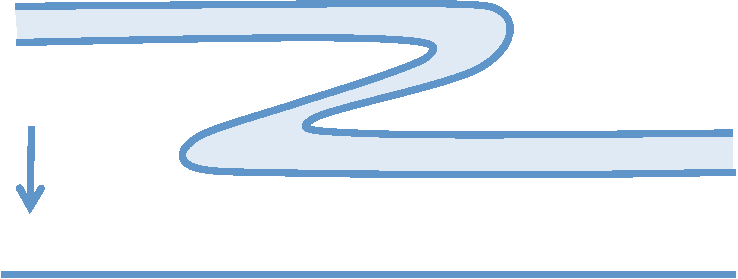
\includegraphics[width=.7\textwidth]{evade_sketch.pdf}
\caption{Is There a Section?}
\label{fig:evade_sec}
\end{figure}

The answer is clearly no. The example in Figure \ref{fig:evade_sec} illustrates a concept central to sheaf theory. Although about each point in time $t$ there is some $\epsilon>0$ such that on the open set $(t-\epsilon,t+\epsilon)$ a continuous section can be defined, there is no globally defined section. Thus local sections (local solutions) exist, but they do not always glue together to define a global section (global solution). This is why we say
\begin{quote}
	\begin{center}
	\emph{Sheaves mediate the passage from local to global.}
\end{center}
\end{quote}

\begin{ex}[Square Map]
	Suppose $f:\CC\to\CC$ is the map sending a complex number $z$ to $z^2$. For a  point $w=re^{i\theta}$ with $r\neq 0$ there are two points in the fiber: $z=\sqrt{r}e^{i\theta/2}$ and $z'=\sqrt{r}e^{i\theta/2 +\pi}$. Consequently, for a small connected neighborhood about $w$ there are two corresponding continuous sections. There is no global section because the square root map is necessarily multi-valued when considered all the whole complex plane.
\end{ex}

Lists of similar examples abound in geometry and topology, most of which are concerned with the following mathematical structure.

\begin{defn}\label{defn:fiber_bundle}\index{fiber bundle}\index{covering space}
A \textbf{fiber bundle} over $X$ consists of total space $E$ equipped with a continuous surjective map $\pi:E\to X$ satisfying the property that for each point $x\in X$ there exists an open neighborhood $U$ such that the following diagram commutes.
\[
\xymatrix{\pi^{-1}(U) \ar[rr]^{h_U} \ar[rd]_{\pi} & & U\times F \ar[ld]^{\pi_U} \\ & U & } 
\]
Here $F$ is the fiber space, $h_U$ is a homeomorphism and $\pi_U$ is projection onto the first factor. If $F$ is a discrete space then we usually write $\tilde{X}$ instead of $E$ and say that $\pi:\tilde{X}\to X$ is a \textbf{covering space}. If each fiber $\pi^{-1}(x)$ is endowed with the structure of a group, i.e. $F=G$ with the discrete topology, so that $h_U$ induces a group isomorphism between $\pi^{-1}(x)$ and $G$, then $E$ is called a \textbf{bundle of groups}. Analogous definitions hold for fiber a ring or a module.
\end{defn}

\index{M\"obius bundle}
The map $\pi:M\to S^1$ where $M:=S^1\times \RR/\sim$ with $(x,y)\sim (x+2\pi,-y)$ is an example of a fiber bundle over $S^1$. Restricting the domain of $\pi$ to the subspace $S^1\times [-1,1]$ allows one to think of this map as projecting the M\"obius bundle to its core circle. The projection $\pi$ has a section that embeds $S^1$ as the zero section, but there are no sections which avoid $S^1\times\{0\}$. The ``hairy ball'' theorem is the analogous statement except for the tangent bundle to the two sphere $S^2$. Sheaf theory is the \emph{lingua franca} for bundle theory and category theory. Thus even the most trivial example of a product bundle, $E=X\times k\to X$ where $k$ is a field, is of interest.

\begin{defn}[Constant Sheaf]\label{defn:const_sheaf}\index{sheaf!constant sheaf}\index{sheaf!locally constant sheaf}
	Suppose $A$ is an $R$-module equipped with the discrete topology and $E=X\times A\to X$ is the product bundle. The sheaf of sections of this map is called the \textbf{constant sheaf} $A_X$. If $A=R$ is a field $k$ or the ring $\ZZ$ we will just say the constant sheaf and write $k_X$ or $\ZZ_X$. We will almost always work over a field $k$.
	
	If $\pi:E\to X$ is not necessarily the product bundle, but has fiber $A$, then we call the sheaf of sections of $\pi$ the \textbf{locally constant sheaf} $F$ with value $A$.  
\end{defn}

For locally connected spaces the constant sheaf $k_X$ assigns to any open set $U$ the product of the field $k$ for as many connected components as $U$ has. To see this, let us be more precise about how the algebraic structure of the module/vector space interacts with the topological structure of a fiber bundle~\cite[Sec. 7.2.1]{macpherson-ih-notes}.

\begin{defn}[Local Systems]\label{defn:local_systems}\index{local system}
Let $k$ be a field viewed as a topological space with the discrete topology. 
A \textbf{local system} is a covering space $\pi:L\to X$ equipped with the structure of a $k$-vector space on each fiber. Specifically, an \textbf{$n$-dimensional local system} on a topological space $X$ is a topological space $L$, a map of spaces $\pi:L\to X$, and, for each point $p\in X$, a $k$-vector space structure on $\pi^{-1}(p)$ with the following property: Every point $p\in X$ has a neighborhood $U$ such that there is a homeomorphism $h_U:\pi^{-1}(U)\to U\times k^n$ such that $\pi_U\circ h_U=\pi$ and for each $x\in U$ the vector space structure on $\pi^{-1}(x)$ is induced by $h$ from the one on $\{x\}\times k^n$.
\end{defn}

Our definition of the locally constant sheaf $F$ in Definition~\ref{defn:const_sheaf} is more accurately defined as an $n$-dimensional local system $L$, at least when $A$ is a $k$-vector space. Consider one of the distinguished open neighborhoods $U$ of a point $x\in X$ provided by the definition. Here we have a commutative diagram:
\[
\xymatrix{\pi^{-1}(U) \ar[rr]^{h_U} \ar[rd]_{\pi} & & U\times k^n \ar[ld]^{\pi_U} \\ & U & } 
\]
For a locally connected space we can assume $U$ is connected by replacing $U$ with whatever connected component of $U$ contains $x$. Consider a section of $\pi:L\to X$ over $U$. Since $k^n$ has the discrete topology any section $s$ over $U$ has to be constant since the image of a connected set is always connected. This implies that every section $s$ has the form $h_U\circ s(y)=(y,(v_1,\ldots,v_n))$ for every $y\in U$ and for some fixed vector $\bar{v} \in k^n$. Consequently, for the distinguished neighborhood $U$, the set of sections
\[
F(U)=A_X(U)\cong k^n\cong A.
\]
Moreover, by the local system condition, we can form any linear combination of sections $s_1,s_2\in F(U)$ to obtain a third section $\alpha s_1+\beta s_2\in F(U)$. This implies that the locally constant sheaf is actually a sheaf valued in $\Vect$ --- the category of vector spaces. Arguing in the same way for each connected component tells us that over a union $U'$ of disjoint, connected, distinguished neighborhoods, a locally constant sheaf has the value
\[
F(U')\cong A^{\pi_0(U')} \cong H^0(U';A)\cong H^0(U';k)^n.
\]
This illustrates that a locally constant sheaf can be thought of as taking $H^0$ of a space with ``twisted'' coefficients.

\section{Local Systems: A Bridge Between Sheaves and Cosheaves}
\label{subsec:local_systems}

Formulating locally constant sheaves as a twisted $H^0$ presents an obvious dualization in terms of $H_0$. Moreover this duality reaches higher by considering higher cohomology and homology as well. To understand this, we will need to understand local systems better. 

\begin{defn}\index{local system}\index{category! of local systems}
The collection of local systems over $X$ forms a category $\LocSys(X)$. A morphism of between two local systems $\pi:L\to X$ and $\pi':L'\to X$ is a map $\varphi:L\to L'$ such that $\pi'\circ \varphi =\pi$ and the restricted map $\varphi_x:\pi^{-1}(x)\to \pi^{'-1}(x)$ is a linear transformation.
\end{defn}

The following theorem is classical and allows us to use two definition of local systems interchangeably.

\begin{thm}\index{local system!representation of $\pijuan(X)$}\index{fundamental groupoid $\pijuan(X)$!local systems}\index{representation!of fund@$\pijuan(X)$}
If $X$ is a locally connected and locally simply connected space, then the category of local systems is equivalent to the category of representations of the fundamental groupoid of $X$, i.e. 
\[
\LocSys(X)\simeq \Rep(\pijuan(X)).
\]
Recall that the objects of $\Rep(\pijuan(X))$ are functors $\cL:\pijuan(X)\to \Vect$.
\end{thm}
\begin{rmk}
For a connected space $X$ fixing a base point $x_0$ provides a skeletal subcategory $\pijuan(X;x_0)\hookrightarrow \pijuan(X)$. Precomposing $\cL$ with this inclusion defines a representation of the fundamental group $\pijuan(X;x_0)$.
\end{rmk}
\begin{proof}[Proof (Idea)]
The functor that realizes this equivalence is very easy to describe. Given a local system $L$ one defines a representation $\cL:\pijuan(X)\to\Vect$ by assigning to points $x\in X$, the vector space $\pi^{-1}(x)=:\cL(x)$. Now suppose $\gamma:[0,1]\to X$ is a path connecting $x$ to $y$. Since $\pi:L\to X$ is a covering space, there is a unique lift $\tilde{\gamma}$ connecting any element of $\pi^{-1}(x)$ to an element in $\pi^{-1}(y)$. These lifts piece together to define a \textbf{monodromy map} $\mu_{\gamma}:\cL(x)\to\cL(y)$. Since local systems are fiber bundles, a homotopy of paths pulls back to a trivial bundle, which shows that the map $\mu_{\gamma}$ is invariant under homotopy classes of paths rel endpoints.

Moreover, one can construct a space associated to a functor $\cL:\pijuan(X)\to\Vect$ by considering the product $L:=\prod_{x\in X}\cL(x)$ and topologizing suitably. For example, one could consider a basis of open sets around a point $v\in \cL(x)$ given by the collection of elements $\{w\in L\,|\,\exists\gamma, s.t. \mu_{\gamma}(v)=w\}$. This construction mirrors the usual construction of a classifying space given in Hatcher~\cite[Sec. 1.3]{hatcher} or Munkres~\cite[Ch. 13]{munkres}.
\end{proof}

\begin{figure}
\centering
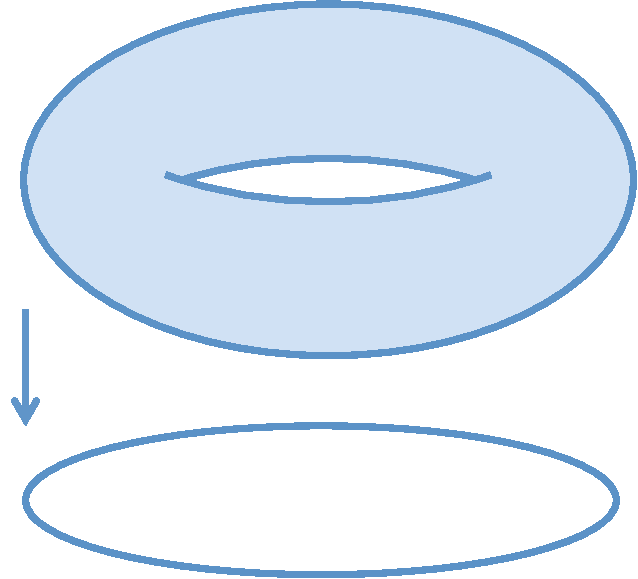
\includegraphics[width=.6\textwidth]{circle_bundle_shaded.pdf}
\caption{Trivial Circle Bundle over the Circle}
\label{fig:circle_bundle}
\end{figure}

This equivalence allows us to define plenty of examples of local systems coming from fiber bundles.
\begin{prop}[Fiber Bundles Give Local Systems]\label{prop:bundles_locsys}\index{fiber byndle!gives local systems}\index{local system!from a fiber bundle}
	Suppose $\pi:E\to X$ is a fiber bundle, then for each $i$ the homology of the fiber $H_i(\pi^{-1}(x);k)$ defines a local system. Dually, for each $i$ the cohomology of the fiber $H^i(\pi^{-1}(x);k)$ defines a representation of the fundamental groupoid and consequently a local system.
\end{prop}
\begin{proof}
	This is easily seen because any path $\gamma:[0,1]\to X$ determines a pullback bundle $\gamma^*E$ which is trivial, so there is an isomorphism $H_i(\pi^{-1}(\gamma(0));k)\to H_i(\pi^{-1}(\gamma(1));k)$. Moreover, any homotopy of paths $H:[0,1]^2\to X$ determines a trivial pullback bundle $H^*E$.
\end{proof}

\index{local system! Klein bottle and torus examples}
Let us now consider two examples. Firstly, in Figure~\ref{fig:circle_bundle} we drew a map from the torus to a circle. To define this map one considers the torus as the space $S^1\times S^1$ and defines the map to be projection onto the first factor. Secondly, consider the analogous projection map from the Klein bottle to the circle. An identification space model is depicted for both of these maps are drawn in Figure~\ref{fig:torus_klein_id} with the left hand side being the torus with its map and the right hand side being the Klein bottle with its map.

\begin{figure}
\centering
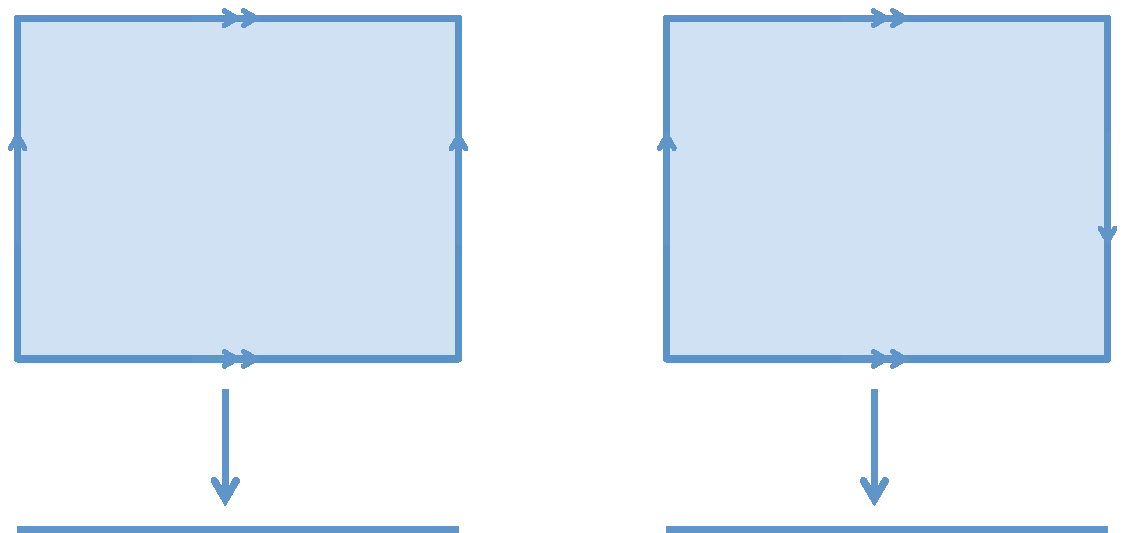
\includegraphics[width=\textwidth]{torus_klein_id.pdf}
\caption{Identification Spaces for the Torus and Klein Bottle}
\label{fig:torus_klein_id}
\end{figure}

Consider the local system gotten by taking $H_1(-;k)$ of the fiber $\pi_T:T\to S^1$. Between any two points $s$ and $s'$ there are two homotopy classes of paths connecting them: one that in the identification space model proceeds directly from $s$ to $s'$ and one that wraps around the circle using the implied identification. Choosing a basis for the vector space $H_1(\pi_T^{-1}(-);k)$ involves choosing a cycle along with an orientation. If one considers the monodromy map associated to either path, one can see that in the bases indicated for $H_1(\pi_T^{-1}(s);k)$ and $H_1(\pi_T^{-1}(s');k)$ in Figure~\ref{fig:torus_action} both monodromies are trivial (i.e. the identity map $k\to k$) as indicated by the green arrows.

\begin{figure}
\centering
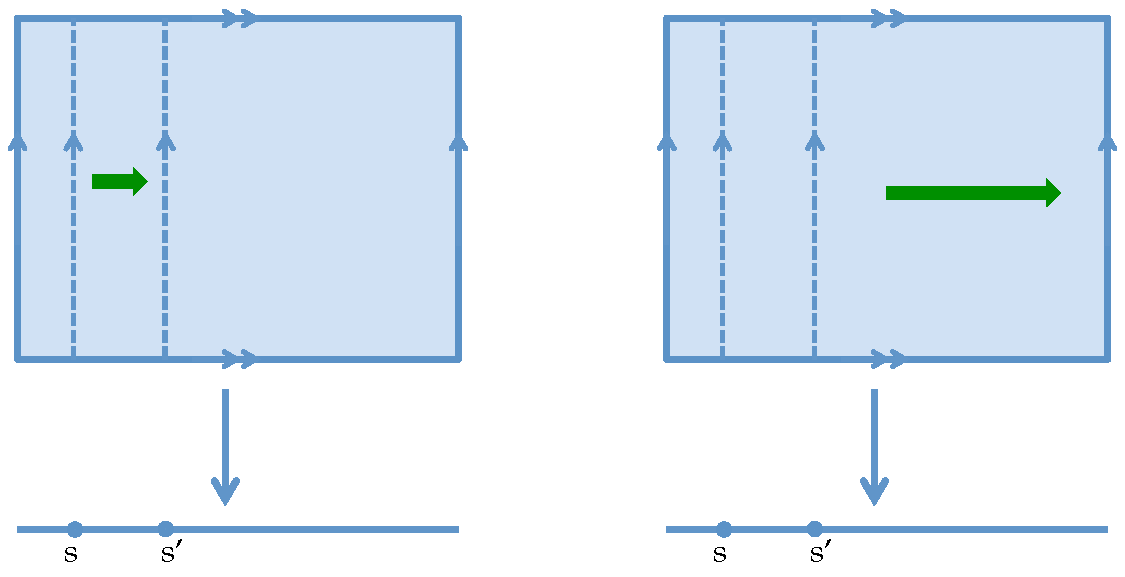
\includegraphics[width=\textwidth]{torus_action.pdf}
\caption{Trivial Action with the Torus Map}
\label{fig:torus_action}
\end{figure}

Now consider the local system gotten by taking $H_1(-;k)$ of the fiber for $\pi_K:K\to S^1$. Choosing the same bases as before the monodromy associated to the longer path that wraps around the identification space is non-trivial
\[
\xymatrix{ H_1(\pi_K^{-1}(s');k) = k \ar[r]^{-1} & k = H_1(\pi_K^{-1}(s);k)}
\]
as indicated by the red arrows in Figure~\ref{fig:klein_action}.

\begin{figure}
\centering
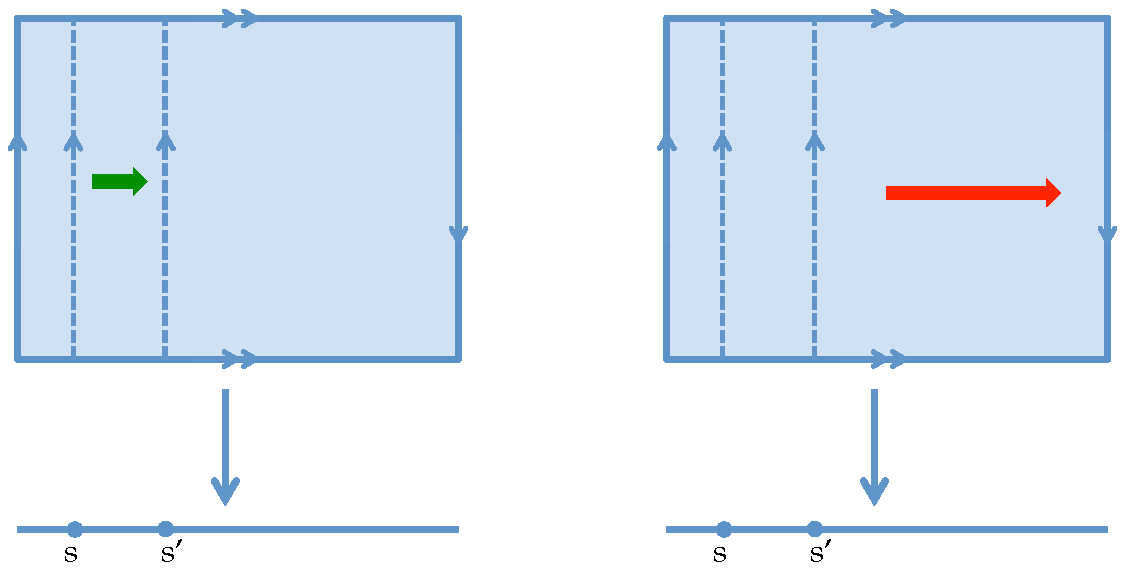
\includegraphics[width=\textwidth]{klein_action.pdf}
\caption{Non-trivial Action from the Klein Bottle}
\label{fig:klein_action}
\end{figure}

We now will show that these examples actually provide examples of locally constant cosheaves, or sheaves if cohomology is taken. First, we will need some alternative definitions.

\begin{defn}\index{sheaf!locally constant sheaf}\index{cosheaf!locally constant cosheaf}
	Let $X$ be a locally connected space. A sheaf $A_X$ or cosheaf $\hat{A}_X$ on $X$ valued in $\Vect$ is \textbf{constant} with value $A$ if for every open set $U$ they make the following assignments:
	\[
	A_X: U \rightsquigarrow A^{\times \pi_0(U)} \qquad \hat{A}_X: U \rightsquigarrow A^{\oplus \pi_0(U)}.
	\]
	A sheaf $F$ or cosheaf $\cF$ is \textbf{locally constant} if for each point $x$ there is an open neighborhood $U$ such that $F$ or $\cF$ is constant, i.e. there is a vector space $A$ such that $F|_U\cong A_X$ or $\cF|_U\cong \hat{A}_X$.
\end{defn}

As a consequence of this definition and the topological assumptions on $X$, a locally constant sheaf or cosheaf possesses for each point $x\in X$ a collection of connected neighborhoods containing $x$ all of which take identical values. As a consequence $F(U)\to F_x$ or $\cF_x \to \cF(U)$ is an isomorphism. Moreover, for any other point $x'$ contained in $U$, the stalk or costalk at $x'$ can be chosen to be isomorphic to $F(U)$ or $\cF(U)$ respectively. By chaining together these sorts of isomorphisms, one can show the following theorem:

\begin{thm}\label{thm:lc_sheaf_rep}\index{sheaf!locally constant sheaf!representation of $\pijuan(X)$}\index{cosheaf!locally constant cosheaf!representation of $\pijuan(X)$}\index{fundamental groupoid $\pijuan(X)$!and locally constant (co)sheaves}\index{representation!of fund@$\pijuan(X)$}
	Suppose $X$ is a locally path connected, locally simply-connected paracompact Hausdorff space. A locally constant sheaf determines a a local system, where a local system is defined to be a representation of the fundamental groupoid of $X$, i.e.
	\[
		\Loc: \pi_1(X) \to \Vect.
	\]
	Similarly, any locally constant cosheaf valued in $\Vect$ determines a local system.
\end{thm}
\begin{proof}
	By taking stalks or costalks we can define the functor $\Loc$ on objects $x\in X$ to be $F_x$ or $\cF_x$, respectively. Since the theorem is well known (see~\cite{achar-lsu} for a proof, which we follow here) for sheaves we present the cosheaf-theoretic proof instead.
	
	Call a subset $K$ of $X$ \emph{fine}\footnote{In~\cite{achar-lsu} they use the word ``good.''} for a cosheaf $\cF$ if it is connected and is contained in a connected open set $V$ such that $\cF|_V$ is a constant cosheaf. For any set of points $\{x_i\}$ in a fine set $K$ we have a collection of isomorphisms
	\[
	\xymatrix{ & \cF(V) & \\
	\cF_{x_i} \ar[ur]^{\pi_i} & \cF_{x_j} \ar[u]^{\pi_j} & \cF_{x_k} \ar[lu]_{\pi_k} }
	\]
	that when composed together allows us to define an invertible map from $\cF_{x_i}\to \cF_{x_k}$ via $\pi_{k}^{-1} \pi_i$. Of course this map agrees with the composition of the analogously defined map $$\cF_{x_i}\to \cF_{x_j} \to \cF_{x_k}$$ because $\pi_k^{-1}\pi_j\pi_j^{-1}\pi_i=\pi_{k}^{-1} \pi_i.$
	
	Now we claim that given a path $\gamma:[0,1]\to X$ there exists a sequence of points $0=a_0< a_1 < \cdots < a_n=1$ so that for all $i$ the set $\gamma([a_i,a_{i+1}])$ is fine. This is the case because every point $\gamma(t)$ possesses a fine neighborhood and by continuity there are open intervals $V_t$ of $t$ such that $\gamma(V_t)$ is fine. If we choose intervals $[a,a']$ contained in each $V_t$, the interiors of these intervals will form an open cover of $[0,1]$. By compactness, finitely many of these intervals will do. Choosing such a finite list, merging and ordering the endpoints, gives the requested sequence.
	
	From the sequence we can define the map $\rho(\gamma):\cF_{\gamma(0)}\to\cF_{\gamma(1)}$ to be the composite
	\[
		\cF_{\gamma(a_0)} \to \cF_{\gamma(a_1)} \to \cdots \to \cF_{\gamma(a_n)}.
	\]
	This map is well defined by virtue of the fact that it is invariant under the addition of extra points $a'$ to the sequence above. Consequently, if any different sequence was chosen we could have merged it with this one and deduced that these maps were the same.
	
	A similar argument can be used to show that for homotopies $H:[0,1]\times [0,1] \to X$ there are sequences $\{a_i\}_{i=1}^n$ and $\{b_j\}_{j=1}^m$ so that the sets $H([a_i,a_{i+1}]\times [b_{j},b_{j+1}])$ are fine. Using the same concatenation of isomorphisms proves that if $\gamma$ and $\gamma'$ are homotopic relative endpoints, then the above defined maps $\cF_{\gamma(0)}\to \cF_{\gamma(1)}$ and $\cF_{\gamma'(0)}\to \cF_{\gamma'(1)}$ are the same.
\end{proof}

Moreover, one can show that representations of the fundamental groupoid give rise to locally constant sheaves and cosheaves. This will require a slightly more sophisticated version of van Kampen's theorem found in~\cite{brown-vkt, may-cat}.

\begin{prop}[van Kampen's Theorem]\index{van Kampen theorem}
	Suppose $X$ is a locally connected topological space, and suppose $\covU=\{U_i\}$ is a cover of $X$ by path-connected open subsets, then the van Kampen theorem states that
	\[
	\pijuan(X)\cong \varinjlim_{I\in N(\covU)} \pijuan(U_I),
	\]
	i.e. the functor $\pi_1:\Open(X)\to\Grpd$ is a cosheaf for the cover $\covU$. However, since any cover is refined by its connected components, which are open by assuming local connectivity, the arguments of Section~\ref{subsec:refinement} imply that the fundamental groupoid is a cosheaf. 
\end{prop}

\begin{thm}\label{thm:rep_lc_sheaf}\index{fundamental groupoid $\pijuan(X)$!determines locally constant (co)sheaves}
	A representation of a fundamental groupoid $\Loc:\pijuan(X)\to\Vect$ determines a locally constant sheaf and a locally constant cosheaf respectively.
\end{thm}
\begin{proof}
	Again the sheaf theoretic version of this statement is well known (see~\cite{achar-lsu}), so we carry out the cosheaf version. Assume we have a local system $\Loc$, then we define the associated cosheaf to be
	\[
	\widehat{L}:U \rightsquigarrow H_0(U;\Loc):=\varinjlim_{x\in U} \Loc|_U,
	\]
	which is a cosheaf on account of the fact that colimits commute with colimits. The fact that $\widehat{L}$ is locally constant comes from the fact that each point $x$ has a simply connected neighborhood $U$ for which the local system $H_0(U;\Loc)\cong \Loc(x)$ for any $x\in U$.
	
	Although it is not pointed out in the literature, the classical proof for sheaves follows by making the exact dual assignment.
	\[
		L: U \rightsquigarrow H^0(U;\Loc):=\varprojlim_{x\in U} \Loc|_U
	\]
\end{proof}
\begin{rmk}[Alternative Proof]
	The introduction of an apparently superfluous $H_0(-;\Loc)$ is an invocation of the principle that $H_0$ is a cosheaf. This principle, expressed in Theorem \ref{thm:MV_cosheaf}, actually states that ``$H_0$ for any homology theory that satisfies Mayer-Vietoris is a cosheaf.'' This is true again for this case, but it requires that the reader know that local systems allow us to define a homology theory with ``twisted coefficients.'' This theory, which uses singular chains with coefficients determined by $\Loc$, satisfies the Eilenberg-Steenrod axioms~\cite[Ch.~6]{whitehead} and thus Mayer-Vietoris~\cite[Ch.~4.6]{spanier}. To complete our alternative proof of the above theorem, we check one more hypothesis of Theorem \ref{thm:MV_cosheaf}. We observe that for an upward increasing sequence of open sets $\{U_i\}$ we have a directed system of chain complexes of twisted singular chains whose right most end point looks like the (non-exact) sequence
	\[
		C_1(U_i;\Loc) \to C_0(U_i;\Loc) \to 0.
	\]
	Taking $H_0$ involves only taking a cokernel, which commutes with direct limits. This proves that $H_0(-;\Loc)$ is a cosheaf.
\end{rmk}

This establishes the following corollary, justifying that local systems do indeed form a bridge between locally constant sheaves and cosheaves.

\begin{cor}
With the above topological assumptions on $X$, the category of locally constant sheaves and locally constant cosheaves are equivalent.
\end{cor}

We leave the details to the reader, who should note that any local system $\cL$ defines a sheaf by taking $H^0(-;\cL)$ and a cosheaf by taking $H_0(-;\cL)$.

\section{Cosheaves Model Topology}

The omnipresence of sheaves in geometry and topology should come with no surprise to many researchers in the algebraic cousins of these fields. Remarkably, cosheaves are just as abundant, but this fact is less well appreciated. This might stem from a desire to avoid excessive terminology as very classical constructions in topology might be called cosheaves, but we will briefly reverse this wisdom to provide ourselves with lots of examples.

Perhaps the closest parallel to the sheaf of sections is the cosheaf of pre-images, but the presence of topology makes it a richer object of study.

\begin{defn}[Cosheaf of Pre-images]\index{cosheaf!of pre-images}
	Suppose $f:Y\to X$ is a continuous map. We can define the pre-cosheaf of topological spaces $\hF:\Open(X)\to\Top$ by assigning to an open subset the pre-image $f^{-1}(U)\in\Open(Y)$ endowed with the subspace topology, i.e.
	\[
	U \rightsquigarrow f^{-1}(U).
	\]
	Since colimits in the open set category are just unions and $f^{-1}(\cup_i U_i)=\cup_i f^{-1}(U_i)$, this defines a cosheaf.
\end{defn}

\begin{ex}[Feature Function]\index{cosheaf!of features}
	Suppose we have a topological space $X$, populated with features of interest, expressed as a function $P:\{1,\ldots, n\}\to X$. We get a cosheaf of sets via $\hF(U)=P^{-1}(U)$. A slightly different cosheaf is gotten by letting $\hG(U)=U\cap\im(P)$, which cannot distinguish points with identical images.
\end{ex}

In the case $n=1$ we can linearize this last example to define an example analogous to an example commonly encountered when studying sheaves.

\begin{figure}[ht]
\centering
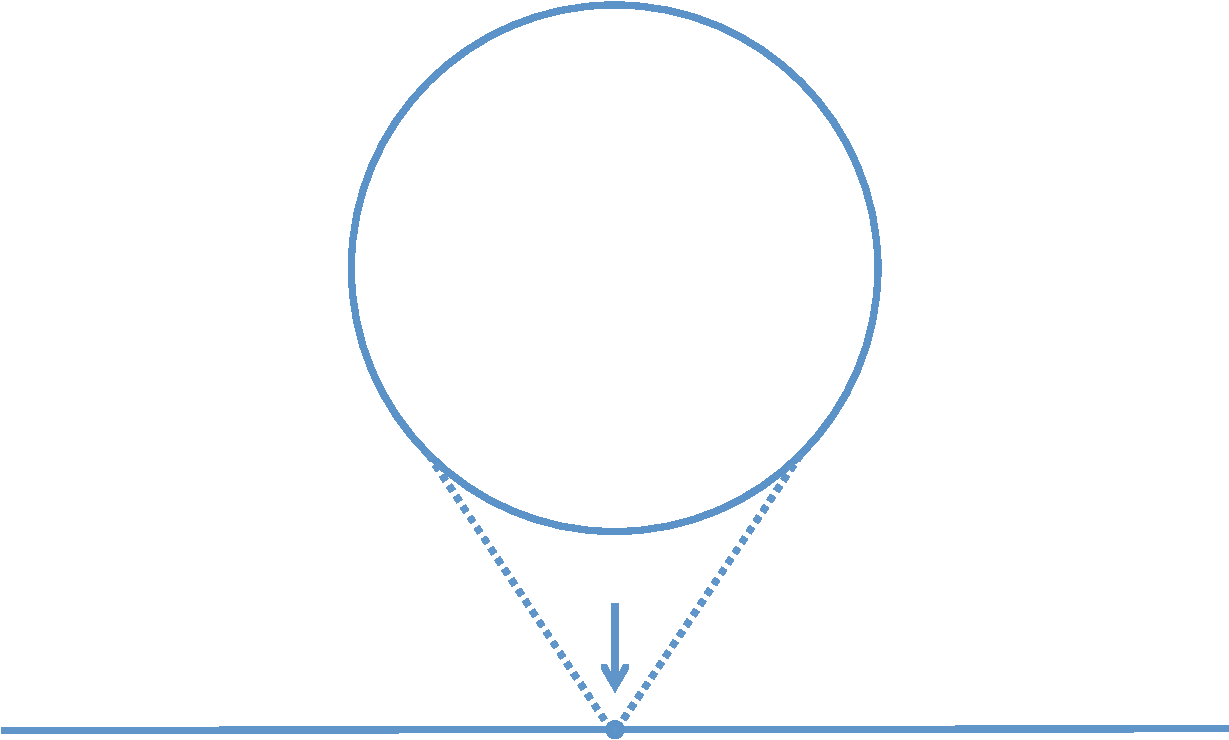
\includegraphics[width=.6\textwidth]{presheaf_2.pdf}
\caption{Topological Model for Skyscraper Cosheaf}
\label{fig:skyscraper}
\end{figure}

\begin{defn}[Skyscraper Cosheaf]\index{cosheaf!skyscraper}
	Suppose $x\in X$ and $V$ is an $k$-vector space. Let's define the \textbf{skyscraper cosheaf} at $x$ with value $V$ to be
	\[
		\skycshv_x^V(U)=\left\{ \begin{array}{ll} V & \textrm{if $x\in U$}\\
		0 & \textrm{otherwise.}\end{array} \right.
	\]
	When $V=k$, we drop the superscript for notational convenience.

	A topological incarnation for the skyscraper is depicted in Figure~\ref{fig:skyscraper}. Here one makes the assignment
	\[
	U \rightsquigarrow H_0(f^{-1}(U);k)
	\]
	where $f$ is the map that maps the circle to the point $x$, i.e. the constant map with value $x$.
\end{defn}

\index{pointless topology}\index{locale}
We could adopt the perspective of cosheaves of pre-images as an alternative to continuous functions. This has been suggested in the past by John von Neumann and his derisively-named \textbf{pointless topology}, where in place of topological spaces one uses the poset of open sets as a primary notion --- an example of a \textbf{locale} --- and one observes that every continuous map of spaces $f:Y\to X$ induces a functor between categories $f^{\circ}:\Open(X)\to\Open(Y)$. This perspective will be of use later as we introduce operations on sheaves and cosheaves.

The cosheaf of pre-images will provide us with lots of examples of cosheaves pertinent to topology. However, viewing the entire information of the fiber (pre-image) is often too much to consider. Instead, one can consider invariants of the fiber and get a sometimes simpler, but still content-rich cosheaf (pending certain properties of the invariant).

\begin{defn}[Cosheaf of Connected Components]\index{cosheaf!of connected components}
	Given a continuous map of spaces $f:Y\to X$, one can define a pre-cosheaf of the components of the pre-image (not path components) $\hF:\Open(X)\to\Set$. This is done via the assignment
	\[
	U \rightsquigarrow \pi_0(f^{-1}(U)).
	\]
	This is not always a cosheaf. However, if $Y$ happens to be locally connected, i.e. the connected components of an open set are open, then it is. Alternatively, one can observe that the functor $\pi_0:\Top_{lc}\to\Set$ is left adjoint to the discrete space functor and so it preserves colimits~\cite{woolf}.
\end{defn}

\begin{ex}[The Square Map, Again]
Consider the cosheaf of connected components associated to the map $f:S^1\to S^1$ defined in complex coordinates as $f(z)=z^2$. For every point $p\in S^1$ there are two connected components in the fiber over $p$. However, there is only one connected component over the whole of $S^1$. This illustrates a sort of ``twisted'' $H_0$ already alluded to.
\end{ex}

\begin{exr}
Work out the cosheaf of connected components associated to the map $\pi:E\to X$ found in Figure~\ref{fig:evade_sec}.
\end{exr}

The next example provides a derived version of the principle that $H_0$ is a cosheaf.

\begin{ex}[Singular p-chains]\index{cosheaf!of singular chains}
	Fix $X$ a topological space and an open subset $U$. A singular p-chain on $U$ is nothing more than a $R$-linear combination of maps of the form $\sigma:\Delta^p\to U$. Since we can always post-compose a $p$-chain on $U$ with an inclusion $U\hookrightarrow V$, this defines a pre-cosheaf
	\[
	C_p(U)=\{\sum_{\sigma} \lambda_{\sigma}\sigma | \lambda_{\sigma}\in R, \sigma:\Delta^p\to U\}.
	\]
	This is, however, not a cosheaf as defined. Try writing down a chain on a union of two open sets as a linear combination of chains on the two sets.
	 A chain needs be sub-divided into pieces coming from each open set, each piece being represented as a map from a fixed simplex. As such, if we define
	\[
	\hat{C}_p(U):=\varinjlim C_p(U)
	\]
	where the colimit is being performed over iterated subdivision, then we obtain a cosheaf~\cite{Bredon}.
\end{ex}

\begin{figure}[ht]
\centering
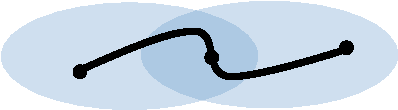
\includegraphics[width=.4\textwidth]{sing.pdf}
\caption{Barycentric Subdivision of a Singular Chain}
\label{fig:sing}
\end{figure}

\begin{rmk}[Mayer-Vietoris and Cosheaves]\index{Mayer-Vietoris!as a cosheaf axiom}
	Another way of seeing that singular $p$-chains do not define a cosheaf is to recall that the proof of the \textbf{Mayer-Vietoris} theorem starts with the observation that the sequence
	\[
	0 \to C_p(U\cap V) \to C_p(U)\oplus C_p(V) \to C_p(U + V) \to 0
	\]
	is exact. Here the $C_p(U+V)$ is just notation for the cokernel of the previous map, thus the sequence is by definition exact. The elements of the cokernel  are linear combinations of singular chains strictly contained in either $U$ or $V$. One then uses barycentric subdivision to show that the \emph{complexes} $C_{\bullet}(U+V)$ and $C_{\bullet}(U \cup V)$ are chain homotopy equivalent. Letting $R=k$ be a field, this motivates defining a cosheaf valued in $\dat=K^b(\Vect_k)$ by assigning
	\[
	U \rightsquigarrow C_{\bullet}(U; k)
	\]
	and this will be a cosheaf.\footnote{The author has recently learned that Jacob Lurie calls this a \textbf{homotopy cosheaf}.} The category $K^b(\Vect_k)$ will be discussed later in the paper where it plays a more important role, but briefly stated it is the category whose objects are chain complexes of vector spaces of finite length and whose morphisms consist of equivalence classes of maps where we have identified those that are chain homotopic. This makes
	\[
		C_{\bullet}(U + V)\cong C_{\bullet}(U\cup V)
	\]
	thereby forcing the cosheaf axiom to hold. Of course the way this isomorphism is proven is via the use of barycentric subdivision, so we can avoid using cosheaves of chain complexes by working with the cosheaf $\hat{C}_p$ directly.
\end{rmk}

The cosheaves of singular chains serve a role precisely dual to the sheaves of co-chains commonly encountered in the literature. Consequently, homology is most naturally associated with cosheaf theory and cohomology is naturally associated with sheaf theory. However, there is a deeper duality between sheaves and cosheaves. When considering compactly-supported cohomology or closed (Borel-Moore) homology the natural habitats reverse. The kernel of this idea is present in the following example.

\begin{ex}[Compactly Supported Functions]\index{cosheaf!of compactly supported functions}
	Suppose $X$ is a locally compact Hausdorff space. Consider the following assignment:
	\[
	\Omega^0_c: U \rightsquigarrow \{f:U\to \RR \,|\, \mathrm{supp}(f) \; \mathrm{compact}\}
	\]
	Compactly supported functions defined locally can always be extended to larger open sets via extension by zero. If $X$ is a manifold, then we get more cosheaves of compactly supported differential $p$-forms $\Omega^p_c$ for $p\geq 0$.
\end{ex}



\section{Taming of the Sheaf... and Cosheaf}
\label{subsec:reeb}

As argued, the canonical example of a sheaf is the sheaf of sections of a map. This stands in contrast with the cosheaf of pre-images. However, a legitimate concern of both examples is its lack of computability. This concern is heightened given that the digital computer is becoming an increasingly common tool for modern mathematics.

A natural question might then be ``Can we store the sheaf of sections on a computer?'' Even in the example depicted in Figure \ref{fig:evade_sec}, it seems unlikely. On a small open set the sheaf of sections is in bijection with the set 
\[
\{f:(x-\epsilon,x+\epsilon)\to (a,b) \, |\, \mathrm{continuous}\},
\] 
which is uncountable. Moreover, for simple spaces like the closed unit interval with its Euclidean topology, there are uncountably many open sets that we need to assign data to.

To handle the first problem of ``too many sections'' in a somewhat ad hoc manner, we can conduct some pre-processing on the input data $\pi:E\to X$. As a motivating example, we can consider a construction normally defined when $X=\RR$.

\begin{defn}[Reeb Graph]\label{defn:reeb_graph}\index{Reeb graph}
	Suppose $Y$ is a topological space and $f:Y\to\RR$ is a continuous map. The \textbf{Reeb graph}~\cite{Reeb} is defined to be the quotient space $R(f):=Y/ \sim$ where $y\sim y'$ if and only if $y$ and $y'$ belong to the same connected component of the fiber $f^{-1}(t)$.
	\[
		\xymatrix{Y \ar[rr]^q \ar[rd]_{f} & & R(f) \ar[ld]^{\pi}\\
		& \RR &}
	\]
	Observe that $R(f)$ still possesses a map to $\RR$. There is clearly a direct generalization for arbitrary base spaces $X$.
\end{defn}

For an example of the Reeb graph, consider our zig-zag from Figure~\ref{fig:evade_sec}. Now let's work out what the sheaf of sections for $R(\pi)$ is and what the cosheaf of connected components is as well. Observe that we can probe the sheaf or the cosheaf on $[0,1]\subset\RR$ by asking what it assigns to open sets of the form $(x-\epsilon,x+\epsilon)$. Clearly it is constant except when the open set intersects a ``critical value.'' We express this observation by assigning values directly to cells in the visible decomposition of the codomain of the function. The data over incident edges and vertices are related, but the direction of that relation is dependent on whether we are considering a sheaf or a cosheaf. Making this observation rigorous has tremendous pay off because it allows us to avoid storing infinitely many open sets by instead working with finitely many cells.

\begin{figure}[ht]
\begin{minipage}[b]{0.47\textwidth}
\centering
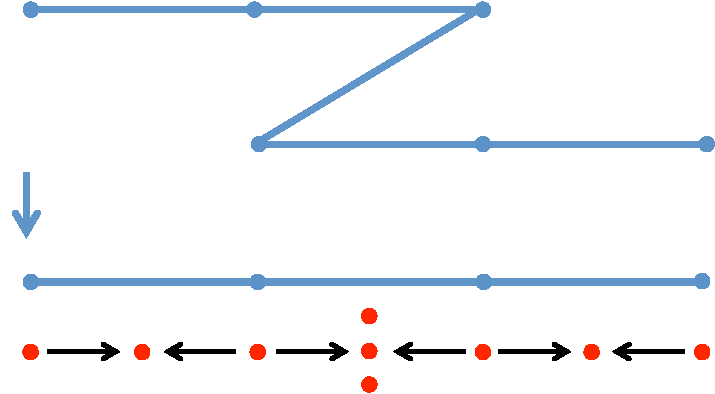
\includegraphics[scale=.6]{evade_sec_reeb.pdf}
\caption{Sheaf of Sections}
\label{fig:evade_sec_reeb}
\end{minipage}
\hfill
\begin{minipage}[b]{0.47\textwidth}
\centering
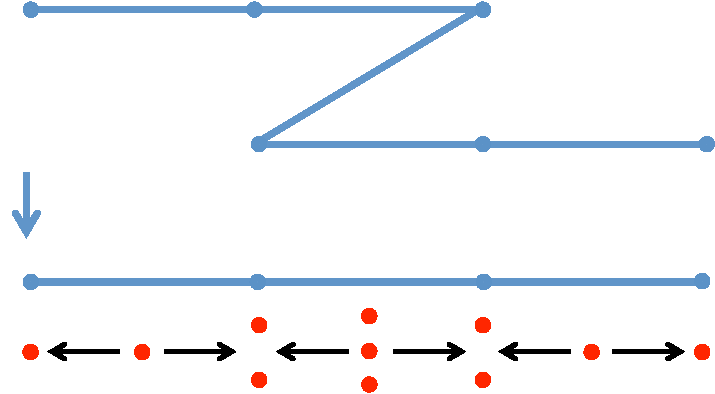
\includegraphics[scale=.6]{evade_comp.pdf}
\caption{Cosheaf of Components}
\label{fig:evade_comp}
\end{minipage}
\end{figure}

